\belowpdfbookmark{Abstract}{sec:abstract}

  \noindent Studies in the field of synthetic biology make constant additions to existing repositories of biological circuits, as well as to the theoretical understanding of their capabilities.
  Although many synthetic gene networks have been demonstrated able to perform computations using biomolecules, until recently the majority of such models were engineered to implement the functionality of single reusable circuit parts.
  \citet{multif} have proposed a network capable of multiple functions, allowing for the selection of three different behaviours in a programmable fashion.
  This work provides an open-source reference implementation with which their \textit{in silico} experiments were replicated.


\section{Introduction}

  The field of biomolecular computing -- and \acs{dna}-based computing in particular -- has advanced remarkably over the last years \cite{history}.
  There are numerous designs of biological parts which implement the behavior of digital logic gates \cite{reconfgate}, continuous-time systems \cite{analog}, oscillators \cite{repressilator}, memory components \cite{register}, asynchronous circuits \cite{async} and so on.
  Such recent developments allow one to consider the possibility of exploting biologically derived materials and their aspects of massive parallelism and self-replication to build practical computing systems on biological \textit{substrata} \cite{youtuber}.

  Amidst forward-engineered biochemical systems, genetic oscillators have been a focus of research \cite{optoscillator} as they are required for the correct operation of synchronous sequential circuits and can also provide persistent periodic \textit{stimuli} to other regulatory networks which may rely on them \cite{bioapps}.
  Genetic switches present another functionality specially useful \cite{bioapps} to digital logic: the ability to toggle between on or off states by either activating or repressing the expression of a certain gene makes them equivalent to a cellular memory unit \cite{youtuber}.
  One study has shown that combining an oscillator with a toggle switch under certain circumstances will result in the generation of a clock-like near square wave signal \cite{clock}.
  Until recently, though, there was no genetic network capable of exhibiting both of these behaviours and alternating between them.

  \citet{multif} presented the \textit{in silico} design of a novel genetic regulatory network which performs frequency division on an oscillating input.
  During experiments, that model was also discovered able to behave as a self-induced oscillator or toggle switch -- thus ressembling the most successful electronic \ac{ic} ever developed, the 555 timer \acs{ic} \cite{ic555}.
  We believe such multi-functionality may lead to more programmable and reusable components in biological computing and this has led to the reproduction of simulations described in that paper on an open-source implementation of the aforementioned model.


\section{Methods}

  The multi-functional synthetic gene network and its dynamics are wholly described in the original study.
  Supplementary material (``File S1'') contains the complete \ac{ode} system that models the genetic circuit under mass-action kinetics.
  The \ac{qssa} exploited to derive the reduced model is also provided, together with all reaction parameterization and initial state of each experiment.
  These factors allowed for an easy replication of the model, even without direct reference to source code or any usage of the proprietary tools (MAPLE and MATLAB) originally employed.

  The \ac{qssa} equations defining the reduced model are given below, where $[X]$ denotes protein concentration.
  Here, $h^+$ and $h^-$ represent activating and repressing Hill functions with Hill coefficient $N$ and half-saturation concentration $k_A$.
  Additional network constants include protein translation rate $k_{tl}$; maximum and unrepressed transcription rates $\beta$ and $P_{tc}$; and degradation rates for mRNA ($\delta_m$) and repressor proteins ($\delta_x$).
  Thus, we borrow the network's mathematical description from the original paper to replicate each of the hereby presented experiments.
  Unless otherwise stated, experimental results on the next section have protein concentrations initially set to $R1 = R2 = 50nM$, $R3 = R4 = 0nM$ and reaction parameters are the same as given in the reference work.

  \begin{equation*}\label{eq:qssa}
    \begin{aligned}
      \dot{[R1]} &= \alpha h^+([I]) h^-([R2]) + \gamma h^-([R3])           - \delta_x [R1] \\
      \dot{[R2]} &= \alpha h^+([I]) h^-([R4]) + \gamma h^-([R3]) h^-([R4]) - \delta_x [R2] \\
      \dot{[R3]} &= \alpha h^+([I]) h^-([R4]) + \gamma h^-([R1])           - \delta_x [R3] \\
      \dot{[R4]} &= \alpha h^+([I]) h^-([R2]) + \gamma h^-([R1]) h^-([R2]) - \delta_x [R4] \\
    \end{aligned}
  \end{equation*}

  \begin{multicols}{2}
    \begin{equation*}
      \begin{aligned}
        h^+([X]) &= \frac{[X]^N}{k_A^N + [X]^N} \\
        h^-([X]) &= \frac{1}{1 + \frac{[X]^N}{k_A^N}} \\
      \end{aligned}
    \end{equation*}

    \columnbreak

    \begin{equation*}
      \begin{aligned}
        \alpha &= \frac{k_{tl} \beta}{\delta_m} \\
        \gamma &= \frac{k_{tl} P_{tc}}{\delta_m} \\
      \end{aligned}
    \end{equation*}
  \end{multicols}

  All numerical simulations were performed in Octave 5.1.0 using Euler's method with a fixed step size of $60$ seconds.
  This differs from MATLAB's \code{ode45} solver which was chosen by \citet{multif}.
  The choice is justified based on the duration of experiments, the shortest of which take at least four days (virtual simulated time) in order to observe a couple of periods on the oscillating output of the frequency divider.
  Due to the different integration methods employed, some numerical mismatch is expected, but qualitative behaviour should remain the same.

  Every deterministic experiment was carried in two systems: one considering the whole set of \ac{ode}s and another with the \ac{qssa} approximation that is used throughout that study.
  Quantitative results shown refer to the full model and deviations between that and the reduced one are highlighted.
  While stochastic simulations are only briefly mentioned on the main text, more details can be found inside supporting information documents (``File S6'').
  The \ac{cles} described therein were implemented with Gaussian noise being generated (with a fixed seed) through the use of built-in Octave functions.


\section{Results}

  \subsection{Frequency Divider}\label{sec:freq-div}

    The network was originally designed as a frequency divider such that the concentrations of repressor proteins oscillate in approximately one half of the input frequency.
    This behaviour can be observed by feeding the model with a continuously oscillating input -- this would be often the case considering existing genetic oscillators \cite{optoscillator} -- but also works with square waves (Figure \ref{fig:freqdiv-square}).

    \begin{figure}[!htb]
      \centering
      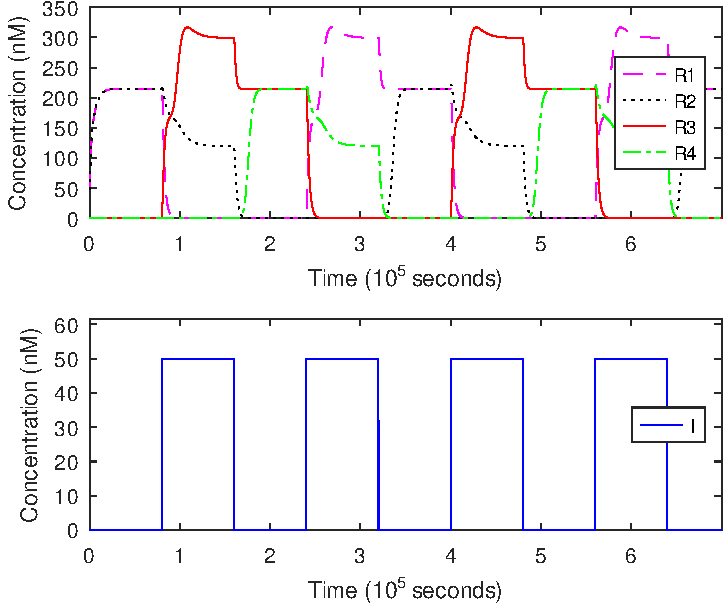
\includegraphics[width=0.8\textwidth]{freqdiv-square}
      \caption{\textbf{Frequency division of clock-like input.} Here we replicate the original paper's Figure 3 with a square wave input with a \SI{50}{\nano M} amplitude, period of $1.6 \times 10^5$ seconds and $50\%$ duty cycle.}
      \label{fig:freqdiv-square}
    \end{figure}

    With a sinusoidal input, output signals from the \ac{qssa} model have constant amplitude, whereas in the full model the first concentration peak of proteins R2 and R3 are higher than the following ones.
    This suggests \acs{mrna} reactions stabilize quicker in the first $10^5$ seconds and thus the approximation is more accurate at those instants \cite{ingalls}.
    After that moment, however, the reduced model exhibits a persistent error in relation to the full one.

    \begin{figure}[!htb]
      \centering
      \begin{subfigure}[t]{0.75\textwidth}
        \centering
        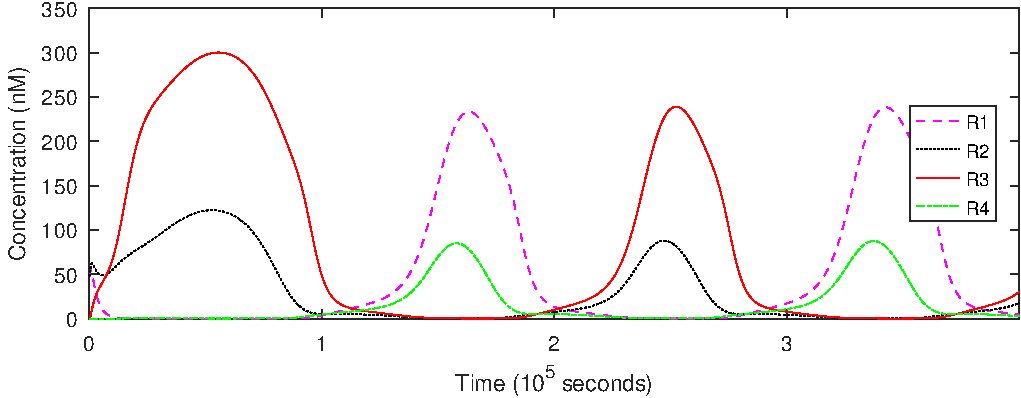
\includegraphics[width=\linewidth]{freqdiv-full}
        \caption{\textbf{Frequency division in the full model.}}
        \label{fig:freqdiv-full}
      \end{subfigure}
      \begin{subfigure}[t]{0.75\textwidth}
        \centering
        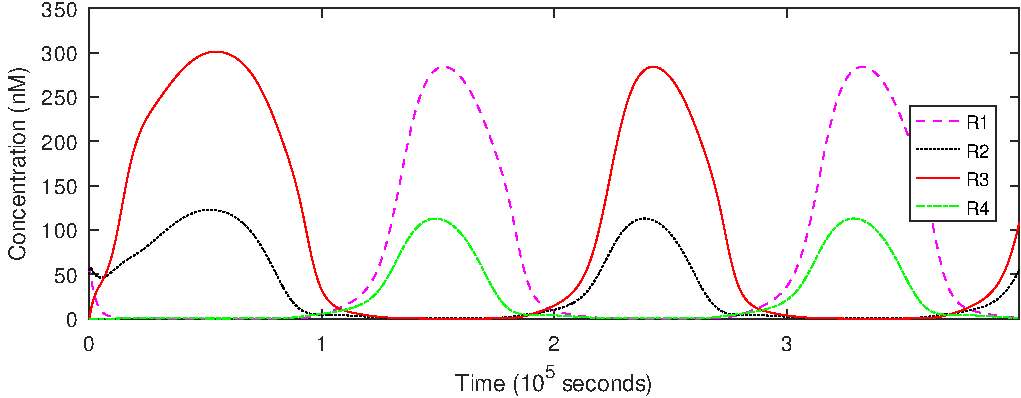
\includegraphics[width=\linewidth]{freqdiv-qssa}
        \caption{\textbf{Frequency division in the reduced model.}}
        \label{fig:freqdiv-qssa}
      \end{subfigure}
      \caption{\textbf{Comparing frequency division between full and reduced models.} This experiment replicates Figure 4 in the reference work. Input varies as a sinusoidal signal with amplitude of \SI{50}{\nano M}, minimum of \SI{6}{\nano M} and a period of $0.9 \times 10^5$ seconds.}
      \label{fig:freqdiv-sine}
    \end{figure}

    As illustrated in Figures \ref{fig:freqdiv-full} and \ref{fig:freqdiv-qssa}, while R1 and R4 concentrations in the full model reach \textit{maxima} valued at \SI{238.29}{\nano M} and \SI{87.62}{\nano M} respectively, the reduced model goes up to \SI{283.96}{\nano M} and \SI{113.05}{\nano M} for each of these proteins (peak values of R3 follow R1 closely and the same happens with R2 and R4).
    This offset distinguishing the two models happens because the \ac{qssa} used to derive the reduced \ac{ode} system considers a separation of time-scales between reactions which regulate \acs{mrna} production and those which describe protein translation.
    In the approximation, the former reactions are assumed to reach equilibrium instantaneously relative to the latter.
    Thus, the difference is a consequence of the fact that the original model maintains itself in a dynamic state that never actually reaches equilibrium \cite{ingalls}, as it perpetually oscillates.

    As mentioned in the original study, frequency division functionality can only be observed after a specific period threshold.
    We ran experiments over a range of input frequencies and found the period-doubling bifurcation to be located near values of $0.8 \times 10^5$ seconds ($\sim 22.22$ hours) in both full and reduced models.
    Although this confirms the network's capability to interface with long-period oscillators, these results -- shown in Figure \ref{fig:freqdiv-period} -- greatly diverge from those in the reference work, which state this threshold could be observed at input periods of approximately $0.275 \times 10^5$ seconds ($\sim 8$ hours).

    \begin{figure}[!htb]
      \centering
      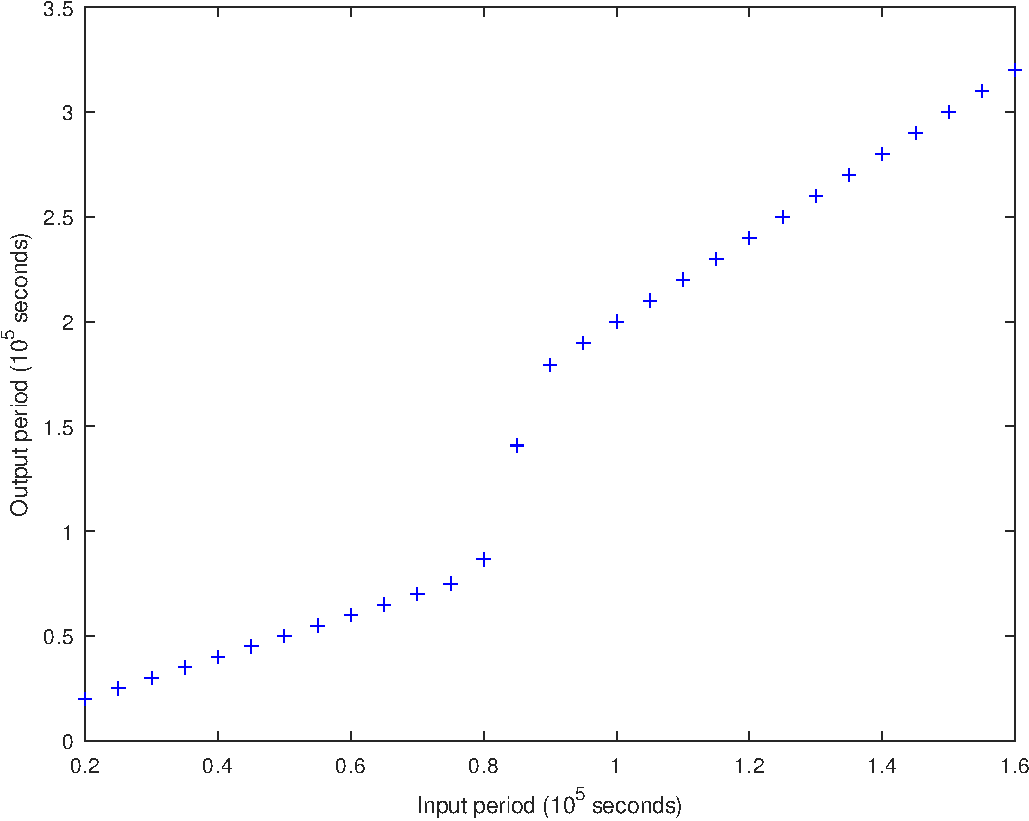
\includegraphics[width=0.85\textwidth]{freqdiv-period}
      \caption{\textbf{Locating the period-doubling bifurcation.} Through this set of successive simulations we attempted to replicate Figure 7A from \citet{multif}. Output period is detected by measuring the distance between R1 concentration peaks. Other than input frequency and simulation length (each run was configured to take as long as five times the input period), parameters are the same as in Figure \ref{fig:freqdiv-full}.}
      \label{fig:freqdiv-period}
    \end{figure}


  \subsection{Bifurcation Analysis}

    \citet{multif} discovered the model's multiple extra functionalities by verifying different behaviours could be attained when input concentration was held constant at specific ranges.
    Experiments regarding the so-called bifurcation analysis were reproduced and Figures \ref{fig:bifurcation-1}-\ref{fig:bifurcation-4} show results under the full model.
    These correspond to the simulation panels displayed within Figure 5 in the reference paper.

    The original study states experiments labeled $4c_{1}$ and $1b$ use the same initial conditions as $4c_{2}$ and $1a$ respectively.
    We believe these were typographical errors, as such settings would lead those pairs of experiments to the exact same results under deterministic semantics and this is not the exhibited behaviour.
    Instead, whereas reaction parameters and input levels are the same as in the original work, initial conditions used are $R1=R2=0nM$ and $R3=R4=50nM$ for experiments $1b$ and $4c_{2}$ and $R1=R2=50nM$ and $R3=R4=0nM$ for all others.

    \begin{figure}[!htb]
      \centering
      \begin{subfigure}[t]{0.45\textwidth}
        \centering
        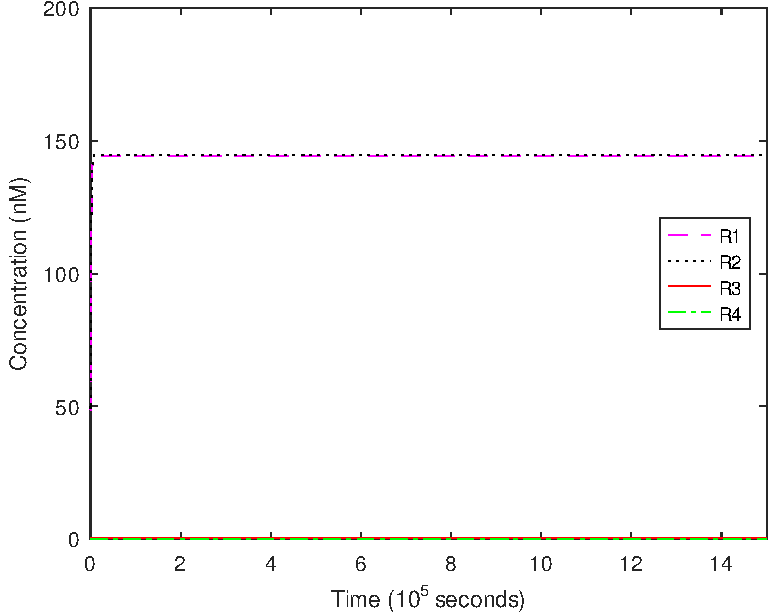
\includegraphics[width=\linewidth]{bifurcation-1a}
        \caption{\textbf{Experiment $1a$.}}
        \label{fig:bifurcation-1a}
      \end{subfigure}
      \hfill
      \begin{subfigure}[t]{0.45\textwidth}
        \centering
        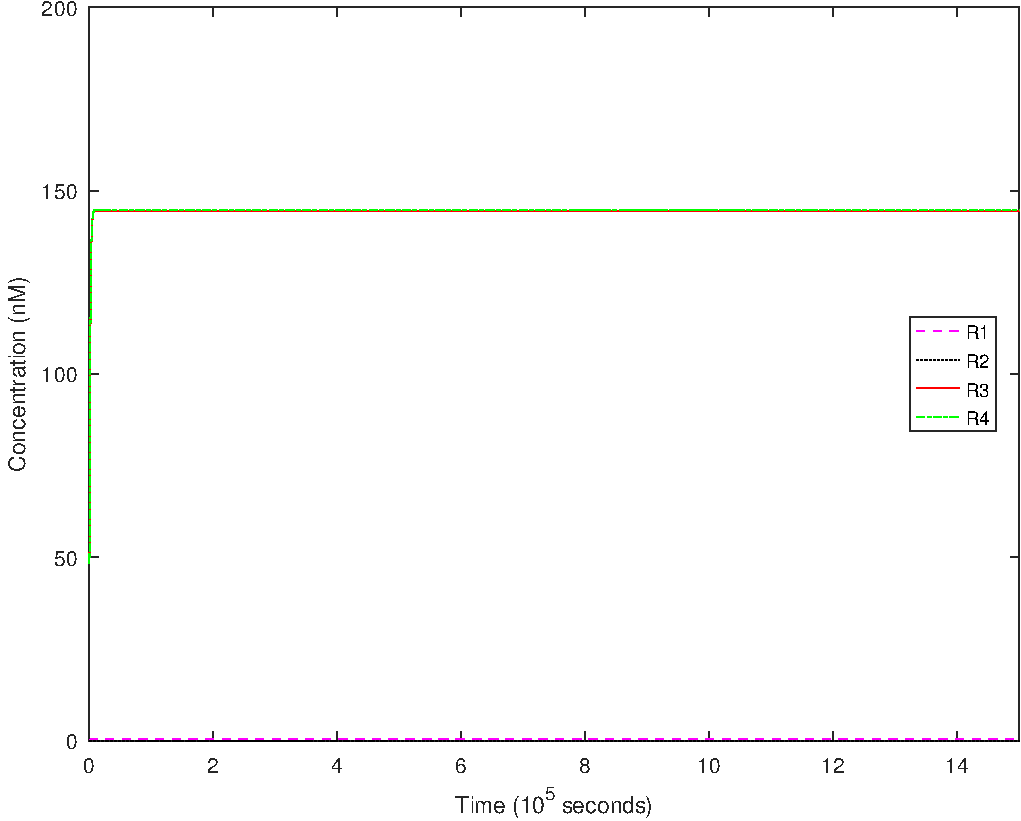
\includegraphics[width=\linewidth]{bifurcation-1b}
        \caption{\textbf{Experiment $1b$.}}
        \label{fig:bifurcation-1b}
      \end{subfigure}
      \caption{\textbf{Low concentration bistable behaviour.} $I = 0.1 nM$.}
      \label{fig:bifurcation-1}
    \end{figure}

    \begin{figure}[!htb]
      \centering
      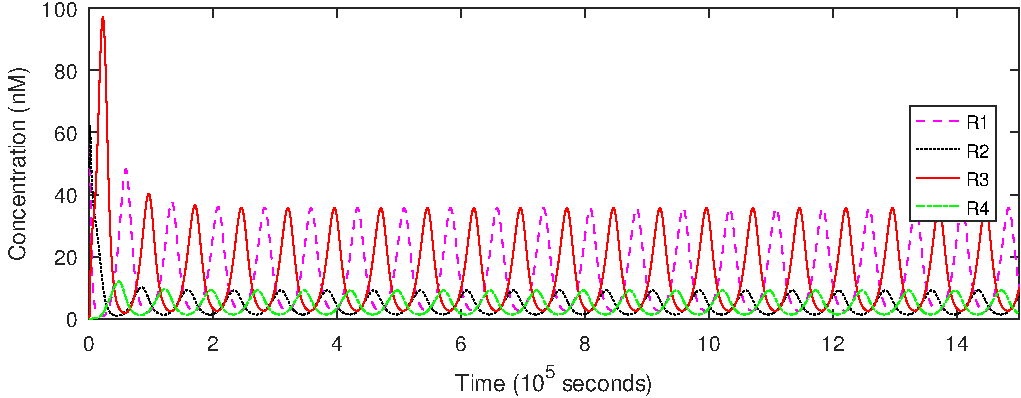
\includegraphics[width=0.7\textwidth]{bifurcation-2}
      \caption{\textbf{Experiment $2$.} $I = 5 nM$.}
      \label{fig:bifurcation-2}
    \end{figure}

    \begin{figure}[!htb]
      \centering
      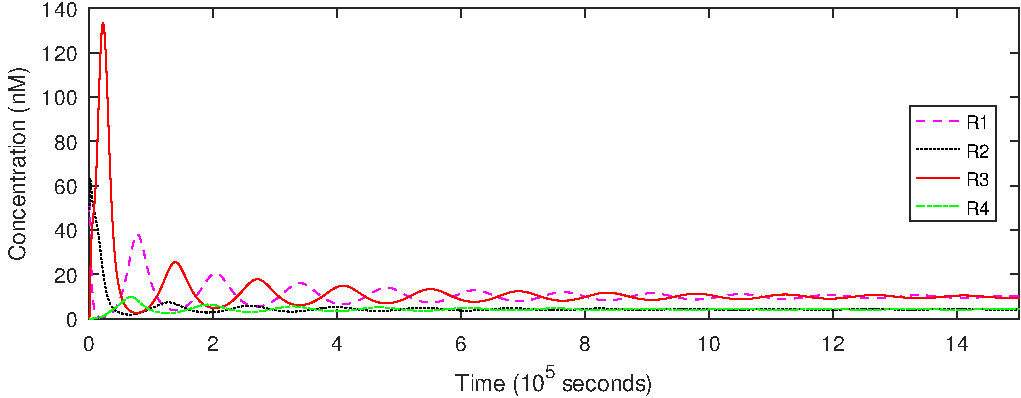
\includegraphics[width=0.7\textwidth]{bifurcation-3}
      \caption{\textbf{Experiment $3$.} $I = 7.5nM$.}
      \label{fig:bifurcation-3}
    \end{figure}

    \begin{figure}[!htb]
      \centering
      \begin{subfigure}[t]{0.45\textwidth}
        \centering
        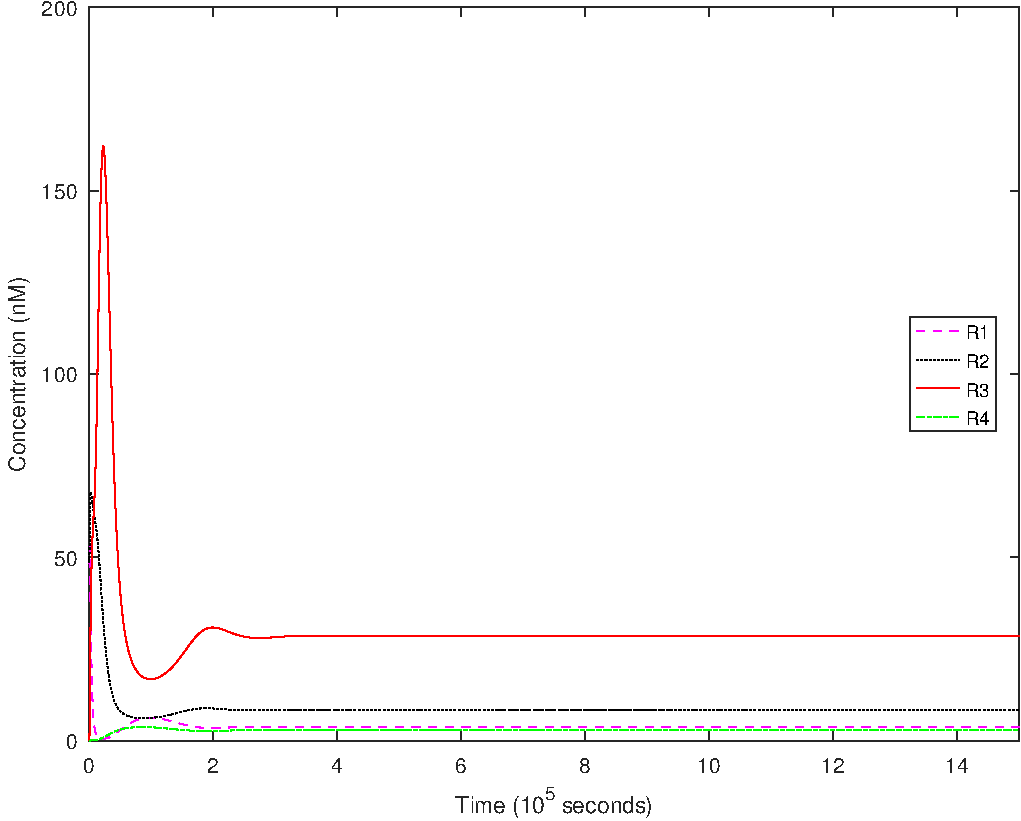
\includegraphics[width=\linewidth]{bifurcation-4c1}
        \caption{\textbf{Experiment $4c_{1}$.}}
        \label{fig:bifurcation-4c1}
      \end{subfigure}
      \hfill
      \begin{subfigure}[t]{0.45\textwidth}
        \centering
        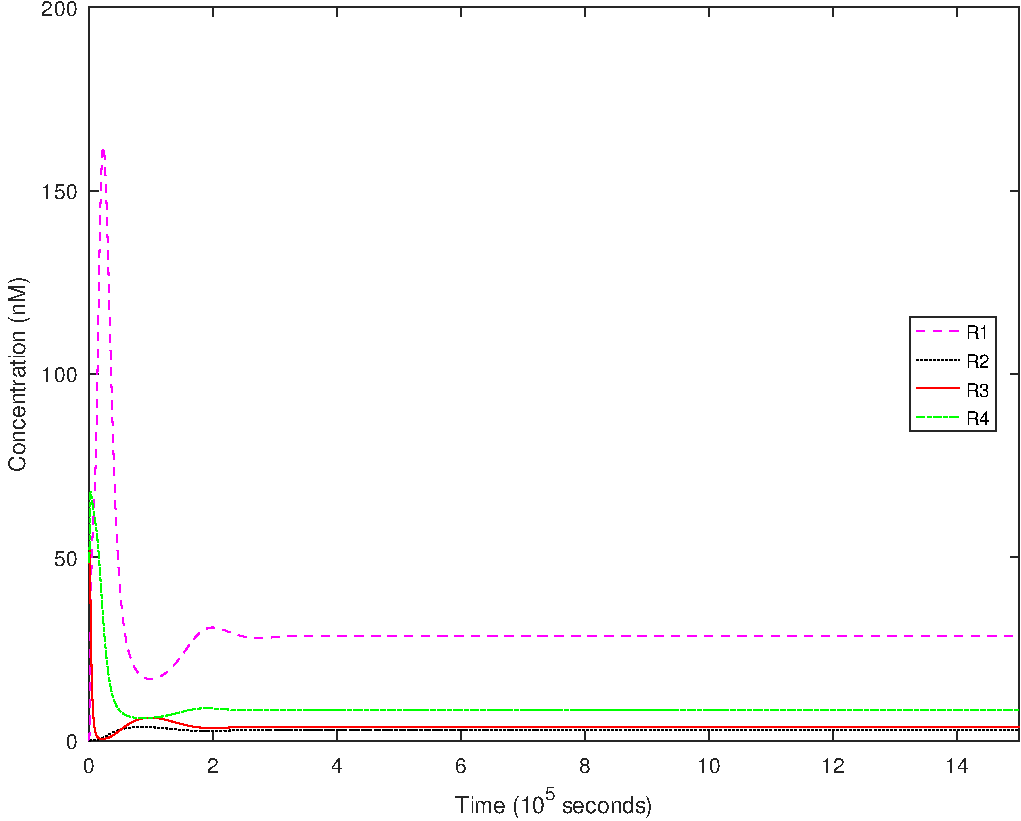
\includegraphics[width=\linewidth]{bifurcation-4c2}
        \caption{\textbf{Experiment $4c_{2}$.}}
        \label{fig:bifurcation-4c2}
      \end{subfigure}
      \caption{\textbf{High concentration bistable behaviour.} $I = 10 nM$.}
      \label{fig:bifurcation-4}
    \end{figure}


  \subsection{Self-induced Oscillator}

    We verified the network's oscillatory dynamics in the region between saddle-node and Hopf bifurcations by measuring its output period for each given input concentration level.
    Results illustrated in our Figure \ref{fig:oscillator-astable} describe a relation with similar behaviour and the same near-vertical increase in period when input approaches the lower bistability region as Figure 6A in the original paper.

    \begin{figure}[!htb]
      \centering
      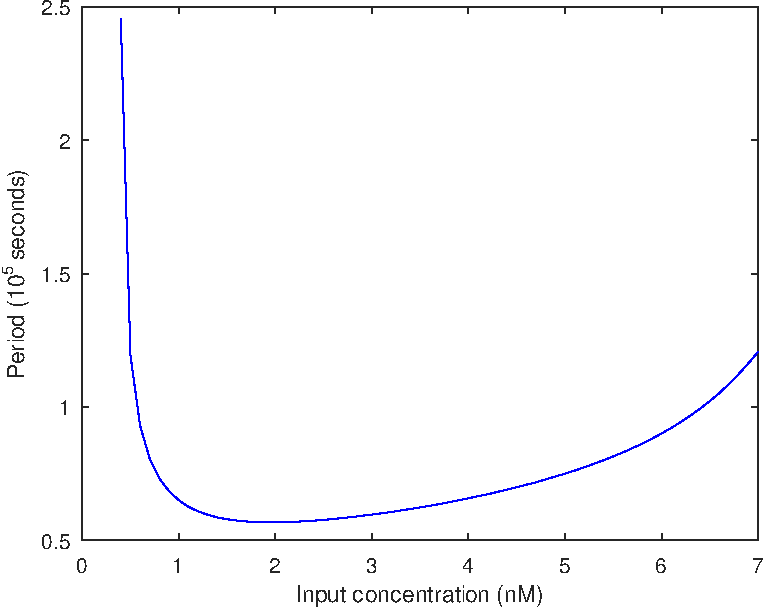
\includegraphics[width=0.76\textwidth]{oscillator-astable}
      \caption{\textbf{Analysing oscillatory dynamics.} Simulation configuration is the same as in Figure \ref{fig:bifurcation-2} except for input levels, which are held in the range $[0.4 nM, 7 nM]$. Output period is detected by measuring the distance between R1 concentration peaks.}
      \label{fig:oscillator-astable}
    \end{figure}


  \subsection{Toggle Switch}

    As revealed during bifurcation analysis, the network exhibits bistability when input concentration is held outside the oscillatory range, that is, at levels lower than \SI{0.4}{\nano M} or greater than \SI{7}{\nano M}.
    Figure \ref{fig:switch} illustrates the system being used as a toggle switch which is ``triggered'' by varying binding affinity of particular repressors, altering $k_A$ momentarily from $6 \times 10^{-10} M$ to $4 \times 10^{-6} M$, as described in the reference work.

    It is important to note that this behaviour can be observed even when the simulated system does not start from a "clean" (i.e. unused) state.
    This means the switch can be toggled on and off repeatedly (not shown), which is to be expected in any non-trivial synthetic biology application \cite{reconfgate}.

    \begin{figure}[!htb]
      \centering
      \begin{subfigure}[t]{0.48\textwidth}
        \centering
        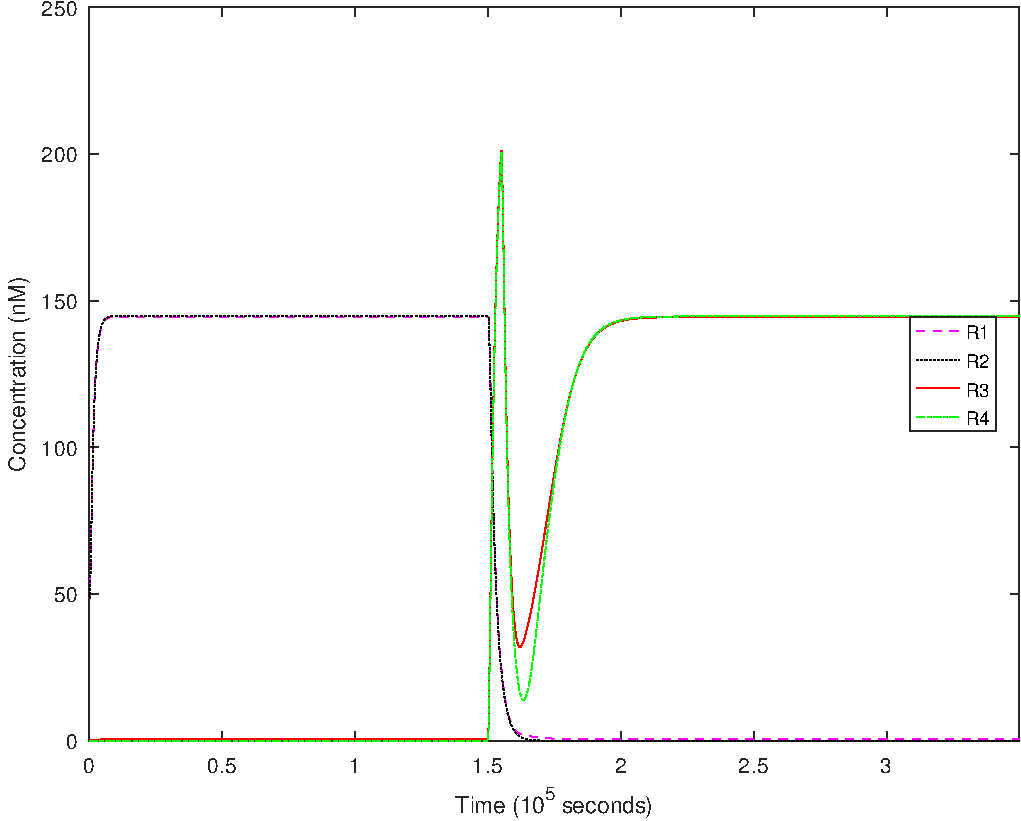
\includegraphics[width=\linewidth]{switch-A}
        \caption{Switching from R1 \& R2 to R3 \& R4 at $I = 0.1 nM$.}
        \label{fig:switch-A}
      \end{subfigure}
      \hfill
      \begin{subfigure}[t]{0.48\textwidth}
        \centering
        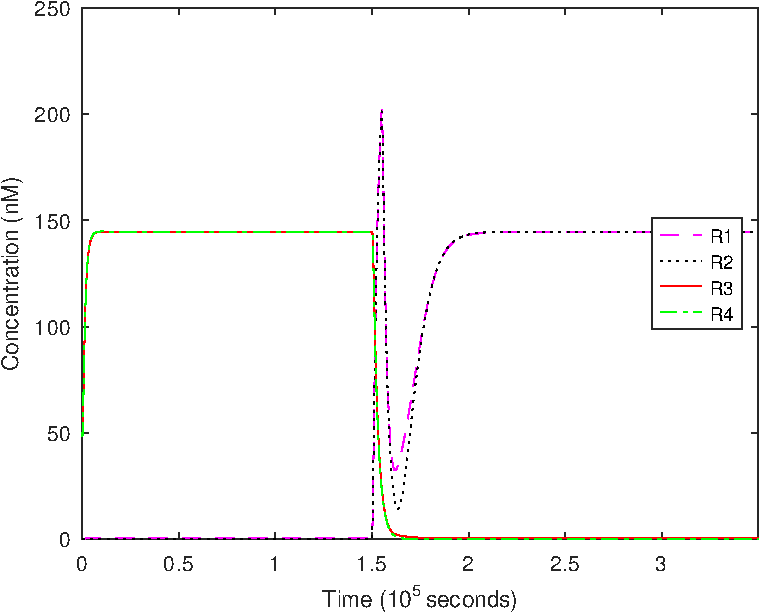
\includegraphics[width=\linewidth]{switch-B}
        \caption{Switching from R3 \& R4 to R1 \& R2 at $I = 0.1 nM$.}
        \label{fig:switch-B}
      \end{subfigure}
      \medskip
      \begin{subfigure}[t]{0.48\textwidth}
        \centering
        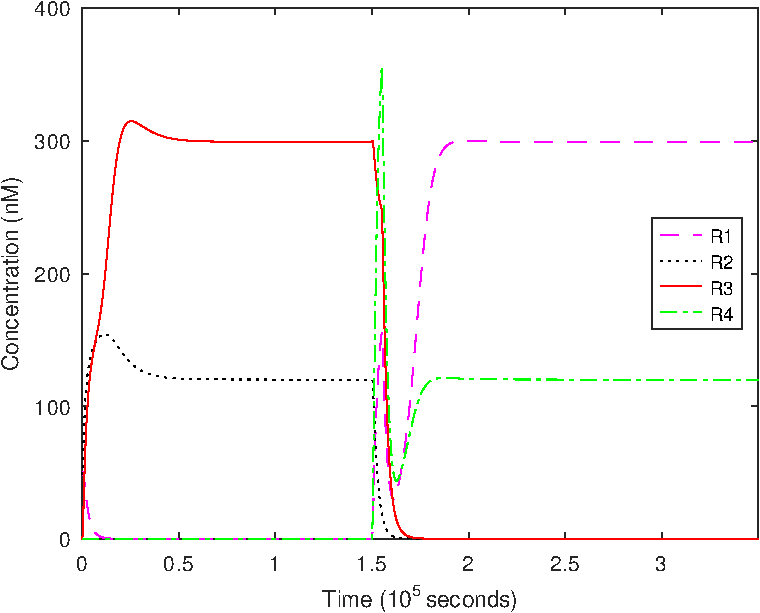
\includegraphics[width=\linewidth]{switch-C}
        \caption{Switching from R2 \& R3 to R1 \& R4 at $I = 50 nM$.}
        \label{fig:switch-C}
      \end{subfigure}
      \hfill
      \begin{subfigure}[t]{0.48\textwidth}
        \centering
        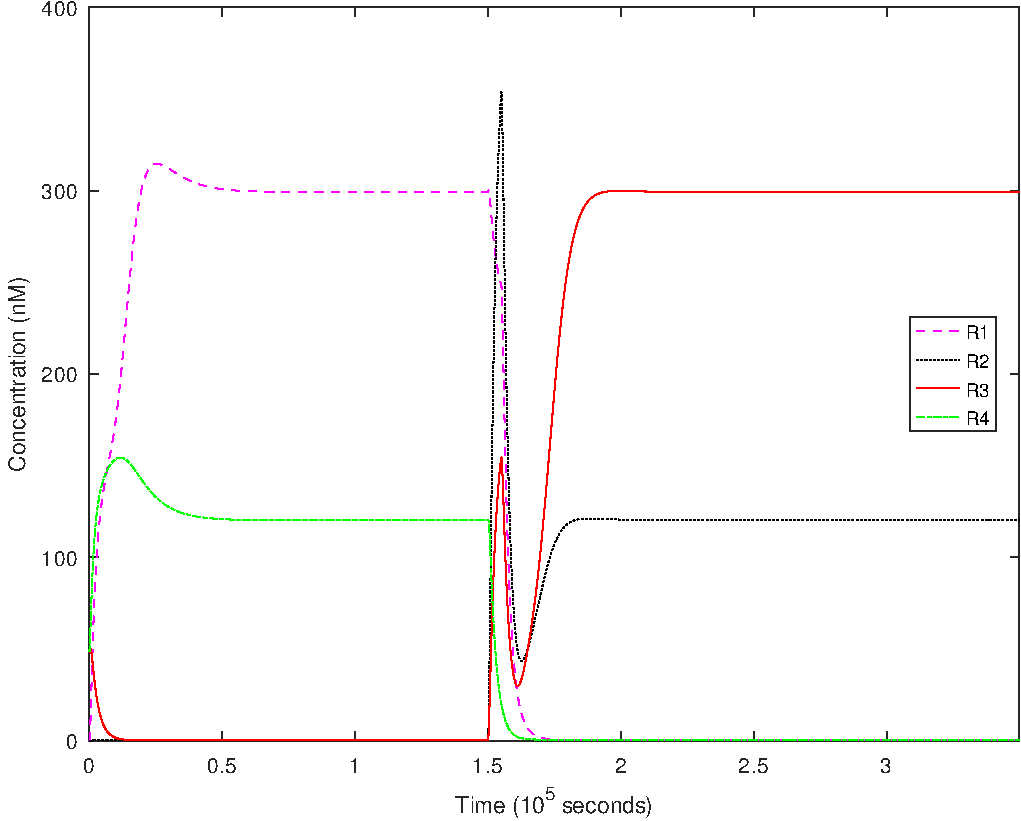
\includegraphics[width=\linewidth]{switch-D}
        \caption{Switching from R1 \& R4 to R2 \& R3 at $I = 50 nM$.}
        \label{fig:switch-D}
      \end{subfigure}
      \caption{\textbf{Demonstrating toggle-switch function.} $k_A$ is altered simultaneously for R1 and R2 in \ref{fig:switch-A} and \ref{fig:switch-C}, while in \ref{fig:switch-B} and \ref{fig:switch-D} the switch is performed by increasing the $k_A$ for R3 and R4. This variation is held between times $1.50 \times 10^5$ and $1.55 \times 10^5$ seconds. Those experiments replicate what is shown in Figure 8 of the reference work.}
      \label{fig:switch}
    \end{figure}


  \subsection{Stochastic Simulations}

    We implemented the \ac{cles} shown in the related supporting information document (``File S6'') provided by \citet{multif}, but it was not possible to verify similar results without modifications to the noise-inducing function.
    While original authors state the usage of Gaussian noise with zero mean and variance of 1, simply employing Octave's \code{randn} function -- which provides such a distribution \cite{randn} -- proved being too noisy as stochastic fluctuations began dominating the model's behaviour.
    It was found through trial and error that downscaling random numbers by a factor of $s \in [\frac{1}{100}, \frac{1}{10}]$ (and consequently scaling variance by $s^2$) would allow for results more similar to those in the reference work.

    \begin{figure}[!htb]
      \centering
      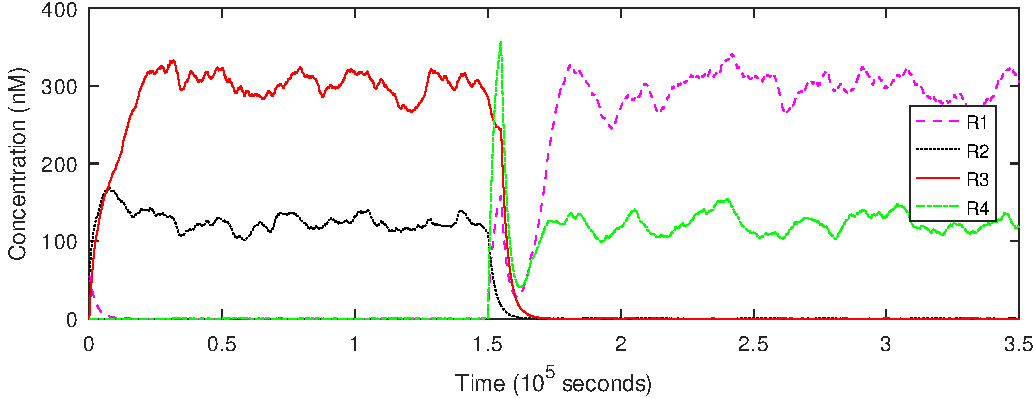
\includegraphics[width=0.8\textwidth]{stochastic-switch}
      \caption{\textbf{Effect of noise on switching function.} Random seed is set to $73544911520192$ and fluctuations are scaled by $\frac{1}{55}$ for a fixed input of \SI{50}{\nano M}.}
      \label{fig:stochastic-switch}
    \end{figure}

    \begin{figure}[!htb]
      \centering
      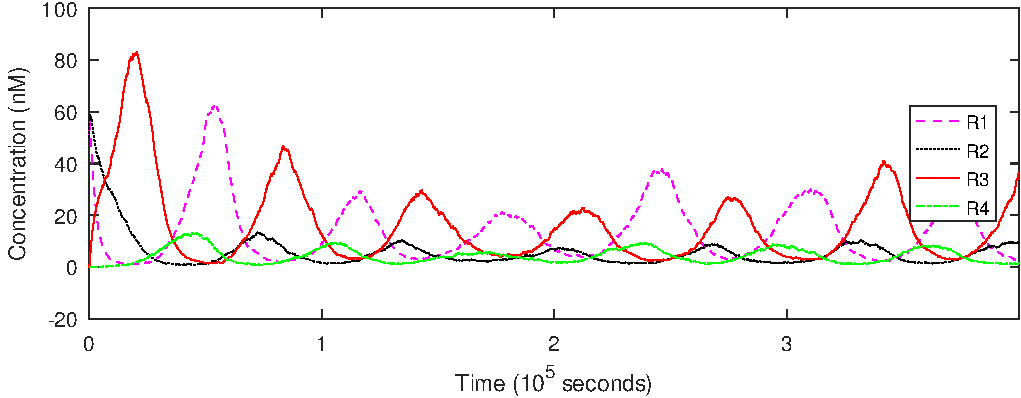
\includegraphics[width=0.8\textwidth]{stochastic-oscillator}
      \caption{\textbf{Effect of noise on oscillator functionality.} Input is set to \SI{5}{\nano M} and noise is scaled by $\frac{1}{55}$. Random seed: $73544911520192$.}
      \label{fig:stochastic-oscillator}
    \end{figure}

    \begin{figure}[!htb]
      \centering
      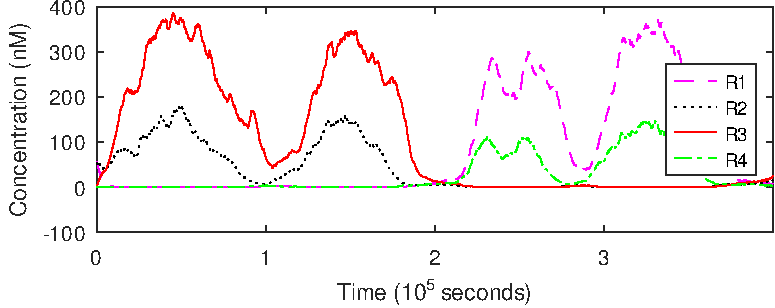
\includegraphics[width=0.8\textwidth]{stochastic-freqdiv-skip}
      \caption{\textbf{Irregular oscillations caused by stochastic fluctuations.} Input is the same as in Figure \ref{fig:freqdiv-full}. Random seed is set to $0.8977812586558097$ and noise is scaled by $\frac{1}{26}$.}
      % scaling = 1/26, seed = 0.8977812586558097 # 2 red, 2 magenta
      % scaling = 1/26, seed = 0.3588309295243656 # 4 red in a row
      % scaling = 1/55, seed = 73544911520192     # expected behaviour
      \label{fig:stochastic-freqdiv-skip}
    \end{figure}

    We verified that among the three functionalities, frequency division possesses less robustness to intrinsic noise: during the stage when input is applied and proteins are all at low concentrations, random fluctuations may cause unintended oscillations as a pair of repressors rise in concentration and prevent transcription of the other two.
    An example of such irregular oscillations is given in Figure \ref{fig:stochastic-freqdiv-skip}, in which a specific random seed and scaling factor pairing that was found to illustrate this behaviour is used.


\section{Conclusions}

  All operation configurations in the multi-functional synthetic gene network were verified and to a large degree the results presented in \cite{multif} were replicated.
  It should be emphasised that the original work stands as an example of reproducible science, with detailed descriptions of model derivation, parameter decisions and extra experiments inside openly available supplementary material.
  Simplifications made using the \ac{qssa} to reduce the full \ac{ode} system proved being a good approximation as even though some small quantitative differences were observed -- and those could be due to the different integration methods as well -- there was no impact on the network's overall dynamics.

  However, stochastic simulations would not provide the expected results without an expressive reduction to noise variance.
  In fact, Gaussian noise seems capable of undermining frequency division functionality to some degree.
  Additionally, the period-doubling bifurcation was empirically found to be at a much lower frequency than what is stated in the reference study.
  Upon correspondence with the authors, it was speculated that some parameter mismatch could have caused this displacement, as qualitative behaviour was mostly maintained.

  We highlight the idea that as synthetic networks grow in complexity and size, multi-functionality may arise more frequently and become difficult to avoid.
  While this can bring the benefits of reusable programmable components, it might also end up becoming a nuisance if models start behaving unexpectedly under the influence of certain inputs.
  At last, we believe further works should focus on a deeper exploration of parameter space.
  The motivation for this is double: it may allow for the characterisation of \textit{in vivo} implementation designs with reusable biological parts and will potentially verify the complete set of specifications for this programmable genetic component and its multiple operating modes.
